\section{LTE}
\label{sec:lte}
\begin{aautop}
    In this part, an overview of the allocated LTE frequency bands will be provided together with a general description of the LTE spectrum.
    In addition to the allocated LTE bands a more detailed description on the bands covered in this project will be provided.
\end{aautop}

\subsection{The History of the Mobile Telephone System}
In this section, an brief overview of the development leading up to 4G and LTE will be given to clarify the need for LTE.

% 1G: 
% - AMPS in US = TACS in UK = MCS-L1 in Japan
% - EU: Different standards for each country [prasad p 5]
% - US: Same all over USA
% - Digital control channel with error-correcting codes
% - Analog voice channels
\subsubsection{1G}
The first generation of mobile phone systems were solely used for speech. In Europe, many different systems were developed and deployed \cite{ramjee1998universal} making it impossible to use the same mobile phones for all of Europe. In USA, the government was in charge of the deployment. For this reason, the AMPS (Advanced Mobile Phone System) was deployed all over the country. The same system was used in England under the name TACS and in Japan under the name MCS-L1 \cite{tanenbaum2012computer}. Because of the US governments interaction, the AMPS system became the most deployed of the first generation system.

AMPS, like the other first generation systems, divided geographical areas into cells, each containing a base station, to which the users transmit, and a Mobile Switching Center which connects the base stations and handles the connections to the phone network. Each cell uses a different set of frequencies than its neighbors, to not avoid interfering with each other. The set of frequencies -- the ``channels'' -- are split into different categories: Control channels for managing of the system, paging channels for alerting the users of incoming calls, access channels for setup and channel assignment, and finally data channels for carrying voice \cite{tanenbaum2012computer}. The data channels are analog voice channels while all other channels are digital (FSK) channels with error-correcting code \cite{tanenbaum2012computer}.

The disadvantages of the first generation of mobile systems included the fact that no world-wide standard existed so mobile phones could only be used in the area for which they were designed. Another disadvantage was that the channels were analog and thus unencrypted. This made eavesdropping possible. The second generation tried to address these problem.

% 2G:
% - Three standards: GSM (EU), D-AMPS (US), and IS-95 (CDMA, Qualcomm)
% - GSM became dominant worldwide 2G
\subsubsection{2G}
In Europe, a lesson had been learned from the first generation system. A single European 2G standard was developed by a telecommunication group -- Groupe Special\'{e} Mobile (GSM). In USA, the task of deploying a second generation mobile system was moved from the government to the marketplace. This resulted in several standards being developed. A digital version of AMPS -- D-AMPS -- was developed. It was designed to coexist with AMPS \cite{tanenbaum2012computer}. A second system, developed by Qualcomm, was described in International Standard IS-95 but was not a dominant 2G system. It did, however, make use of CDMA -- Code Division Multiple Access -- which later became the basis for the third generation of mobile systems. Later on, GSM got deployed in the US as well and has now become the de facto world standard for 2G \cite{ramjee1998universal}.

The major difference from the first to the second generation was the change from analog speech to digitally coded speech. This made it possible to encrypt the speech, addressing the eavesdropping issue of the first generation \cite{tanenbaum2012computer}. Apart from this, the mobile phone and the subscription itself was split into two separate parts. The user would now buy a SIM (Subscriber Identity Module) card which can be used in whatever mobile phone the user desired.

GSM uses frequency bands at around \SI{900}{MHz}, \SI{1800}{MHz}, and \SI{1900}{MHz}. Each band is split into smaller bands (channels), each split into eight time-divided slots so that eight separate connections can be active at the same time \cite{tanenbaum2012computer}. The channels are of two groups -- one for uplink and one for downlink. The channels are illustrated in Figure~\ref{fig:gsmsplitup}. 

Using compression, it is possible for GSM to achieve the equivalent of a \SI{64}{kbps} PCM voice signal with little loss in quality \cite{tanenbaum2012computer}. While this may be fine for speech, a higher data rate would be needed to carry data as well. This led to the development of the third generation.

\begin{figure}[htbp]
    \centering
    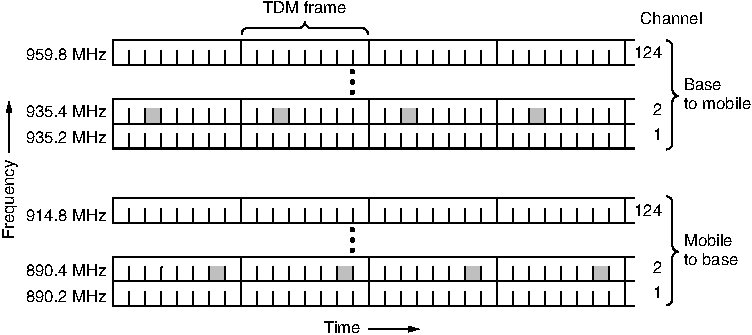
\includegraphics{img/analysis/gsm}
    \caption{Illustration of GSM channels \cite{tanenbaum2012computer}.}
    \label{fig:gsmsplitup}
\end{figure}

% 3G: 
\subsubsection{3G}
The third generation was designed for carrying digital data and speech at higher data rates than previously. Two similar systems were developed in Europe and in USA: UMTS (Universal Mobile Telecommunications System) and CDMA2000, respectively. Europe wanted coexistence with GSM and USA wanted coexistence with IS-95.

The third generation used CDMA as multiple-access scheme. In CDMA, all users communicate the same time, jumping between frequency and time slots in a pre-defined code. The code is shared between transmitter and receiver. Ideally, the codes would be orthogonal so that only one user would communicate on one frequency in one time slot. While this type of synchronization is easily performed in the downlink, it is very difficult in the uplink as the mobile units do not connect directly. Instead, pseudo-random sequences, which can be generated locally, are used as codes. These codes have a low cross-correlation and auto-correlation so that the interference between users is averaged out along the code word \cite{tanenbaum2012computer}.

The transmitted power from the mobile phone in a CDMA system is controlled in a fast loop so that the transmitted power is the inverse of the power received from the base station \cite{tanenbaum2012computer}. This makes the received power from each user equal at the base station, so the interference between users is lowered. 

The CDMA variants used in the third generation of mobile networks makes it possible to assign different data rates to different users. At the same time, these systems can take advantage of periods where a user is not speaking, etc. This will not be described further, but is described in \cite{tanenbaum2012computer}.

The third generation made it possible to obtain a data rate between \SI{144}{kbps} (mobile users) and \SI{2}{Mbps} (indoor users) \cite{tanenbaum2012computer}. HSPA and HSPA+ are evolutions of the UMTS network, enabling higher data rates -- up to \SI{14}{Mbps} and \SI{42}{Mbps}, respectively, pushing the limits of the deployed Wideband CDMA \cite{holma2011lte}. Some of the goals for fourth generation are higher bandwidths and more seamless integration with wired and wireless IP networks \cite{tanenbaum2012computer}. The peak data rate evolution, presented by 3GPP, is illustrated in Figure~\ref{fig:3gppevo}.

\begin{figure}[htbp]
    \centering
    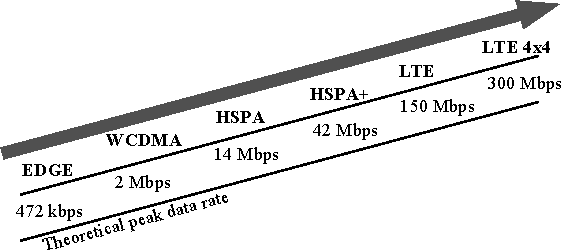
\includegraphics[scale=0.8]{img/analysis/3gppevo.pdf}
    \caption{Peak data rate evolution of 3GPP technologies \cite{holma2011lte}.}
    \label{fig:3gppevo}
\end{figure}

% 2.5G, etc is not covered.

% 4G:
\subsubsection{4G}
LTE (Long Term Evolution) is an evolution of the UMTS, HSPA (High Speed Packet Access), and HSPA+ (Evolved High Speed Packet Access) 3G communication standards. HSPA and HSPA+ are upgrades to UMTS with the primary goal to improve the data rates on the 3G communication network. The LTE standard is marketed as a 4G network, even though the LTE standard does not meet the requirements set by the 4G standard \cite{radio2015electronics}.

The LTE provides much higher data rates than the 3G HSPA+ standard, using Orthogonal Frequency Division Multiplex (OFDM) in downlink and Single Carrier-Frequency Division Multiple Access (SC-FDMA) in uplink. These access scheme technologies do also enable the LTE network to use MIMO technologies, which has resulted in MIMO being an integral part of LTE \cite{radio2015electronics}.

MIMO technologies improves the throughput even further by having the option to add up multipath signals. A further description of MIMO is given in Section~\ref{sec:mimo_in_handsets}. A comparison of the UMTS, HSPA, and LTE speeds can be seen in Figure~\ref{fig:3gppevo}.

% \begin{table}[htbp]
%   \centering
%   \begin{tabular}{|c|c|c|c|c|}
%     \hline
%     & {\bf \begin{tabular}[c]{@{}c@{}}WCDMA\\ (UMTS)\end{tabular}} & {\bf \begin{tabular}[c]{@{}c@{}}HSPA\\ HSDPA/HSUPA\end{tabular}} 
%     & {\bf HSPA+} & {\bf LTE}     \\ \hline
%     {\bf \begin{tabular}[c]{@{}c@{}}Max downlink speed\\ (bps)\end{tabular}} & 384 k & 14 M & 28 M & 100 M \\ \hline
%     {\bf \begin{tabular}[c]{@{}c@{}}Max uplink speed\\ (bps)\end{tabular}} & 128 k & 5.7 M & 11 M & 50 M \\ \hline
%     {\bf \begin{tabular}[c]{@{}c@{}}Latency\\ round trip time\\ approx\end{tabular}} & 150 ms & 100 ms & 50 ms (max) & ~10 ms \\ \hline
%     {\bf Access methodology} & CDMA & CDMA & CDMA & OFDMA/SC-FDMA \\ \hline
%   \end{tabular}
%   \caption{LTE speed specifications \cite{radio2015electronics}.}
%   \label{tab:3g4g_speeds}
% \end{table}

\subsection{LTE Frequency Band Allocation}
As seen in Table~\ref{tab:ltefreqband}, the available LTE bands for uplink and downlink are allocated in the frequencies from \SIrange{452.5}{3600}{MHz}. The whole spectrum between \SIrange{452.5}{3600}{MHz} is not occupied by the mobile communication systems, as other network systems, such as WiFi, GPS, TV, etc., also have the rights (licenses) to some of the frequency bands within this spectrum.

However, the transition from analog to digital broadcast television signals has freed some frequency bands for mobile communication. In USA in 2009, the \SI{700}{MHz} band covering \SIrange{698}{806}{MHz} \cite{fcc2007auction} was auctioned and latest the spectrum around \SI{600}{MHz} has also been freed and was put on auction in 2015 \cite{Samantha2015tunableAntennas}. Furthermore, in 2013 the \SI{800}{MHz} band, which was also freed due to the digital TV transition, and the \SI{2600}{MHz} band were auctioned off by Ofcom \cite{james2014lte}.   

As the mobile communication is evolving, the need for higher data rates also increases, leading to the need for more bandwidth. The freed bands increase the mobile communication spectrum both in the low and high frequencies, which can be used for different environments.  

\subsubsection{High and Low Frequency Bands}
The high and low frequency bands both have advantages and disadvantages. As seen in Table~\ref{tab:ltefreqband}, the bandwidth varies form \SIrange{5}{90}{MHz}; the high frequencies providing high bandwidth and the low frequencies low bandwidth. This means that the high band frequencies provide greater capacity. One of the primary advantages of low band frequencies is the large wavelength. The large wavelength makes the waves able to travel long distances and is suitable for rural areas \cite{pozar2011microwave}. The greater capacity at the high band frequencies makes these bands ideal for communication in urban areas as cities or other dense areas.

\subsubsection{Multiband LTE}
Most countries use several frequency bands across the LTE spectrum, which implies that a multi-band phone/antenna is needed.  
Until now, it has not been possible to agree on the same LTE band allocations across the world because of the different regulatory positions in different countries. Also, in some cases across the different countries, the LTE bands are overlapping as a consequence of different frequency availability around the world, thus limiting the accessibility of all users to use the same frequencies \cite{radio2015electronics}.  

\begin{table}[htbp]
  \centering
  \begin{tabular}{|c|c|c|c|c|c|c|}
    \hline
    \begin{tabular}[c]{@{}c@{}}LTE\\ band\\ number\end{tabular}  & \begin{tabular}[c]{@{}c@{}}Uplink\\ (MHz)\end{tabular} & \begin{tabular}[c]{@{}c@{}}Downlink\\ (MHz)\end{tabular}         & \begin{tabular}[c]{@{}c@{}}Bandwidth \\ (MHz)\end{tabular} & \begin{tabular}[c]{@{}c@{}}Duplex\\ spacing\\ (MHz)\end{tabular} & \begin{tabular}[c]{@{}c@{}}Band \\ Gap\\ (MHz)\end{tabular} & \begin{tabular}[c]{@{}c@{}} Total\\Span\\(MHz)\end{tabular}\\ \hline
    1  & 1920--1980 & 2110--2170 & 60 & 190 & 130 & 250 \\ \hline
    2  & 1850--1910 & 1930--1990 & 60 & 80  & 20  & 140\\ \hline
    3  & 1710--1785 & 1805--1880 & 75 & 95  & 20  & 170\\ \hline
    4  & 1710--1755 & 2110--2155 & 45 & 400  & 355  & 445\\ \hline
    5  & 824--849   & 869--894   & 25 & 45  & 20  & 70\\ \hline
    6  & 830--840   & 875--885   & 10 & 35  & 25  & 55\\ \hline
    7  & 2500--2570 & 2620--2690 & 70 & 120  & 50  & 190\\ \hline
    8  & 880--915   & 925--960   & 35 & 45  & 10  & 80\\ \hline
    9  & 1749.9--1784.9 & 1844.9--1879.9 & 35 & 95  & 60  & 130\\ \hline
    10 & 1710--1770 & 2110--2170 & 60 & 400  & 340  & 460\\ \hline
    11 & 1427.9--1452.9 & 1475.9--1500.9 & 20 & 48  & 28  & 73\\ \hline
    12 & 698--716   & 728--746   & 18 & 30  & 12  & 48\\ \hline
    13 & 777--787   & 746--756   & 10 & $-31$  & 41  & 41\\ \hline
    14 & 788--798   & 758--768   & 10 & $-30$  & 40  & 40\\ \hline
    15 & 1900--1920 & 2600--2620 & 20 & 700  & 680  & 720\\ \hline
    16 & 2010--2025 & 2585--2600 & 15 & 575 & 560 & 590\\ \hline
    17 & 704--716   & 734--746   & 12 & 30  & 18  & 42\\ \hline
    18 & 815--830   & 860--875   & 15 & 45  & 30  & 60\\ \hline
    19 & 830--845   & 875--890   & 15 & 45  & 30  & 60\\ \hline
    20 & 832--862   & 791--821   & 30 & $-41$  & 71  & 71\\ \hline
    21 & 1447.9--1462.9 & 1495.5--1510.9 & 15 & 48  & 33  & 63\\ \hline
    22 & 3410--3500 & 3510--3600 & 90 & 100  & 10  & 190\\ \hline
    23 & 2000--2020 & 2180--2200 & 20 & 180  & 160  & 200\\ \hline
    24 & 1625.5--1660.5 & 1525--1559 & 34 & $-101.5$  & 13  & 135.5\\ \hline
    25 & 1850--1915 & 1930--1995 & 65 & 80  & 15  & 145\\ \hline
    26 & 814--849   & 859--894   & 30/40 &     & 10  & 80\\ \hline
    27 & 807--824   & 852--869   & 17 & 45  & 28  & 62\\ \hline
    28 & 703--748   & 758--803   & 45 & 55  & 10  & 100\\ \hline
    29 & N/A         & 717--728   & 11 &     &     & 11\\ \hline
    30 & 2305--2315 & 2350--2360 & 10 & 45  & 35  & 55\\ \hline
    31 & 452.5--457.5 & 462.5--467 & 5  & 10  & 5   & 14.5\\ \hline
  \end{tabular}
  \caption{LTE frequency band allocation (only frequency division duplex) \cite{radio2015electronics}. Note that negative duplex spacing meas that the uplink band is higher in frequency than the downlink.}
  \label{tab:ltefreqband}
\end{table}

\begin{aautail}
    In this section, an overview of the history of LTE was given. A brief overview of the techniques used in LTE was also given along with a table of the LTE bands currently in use. This gives an overview of what frequency bands the antennas designed in this project needs to cover.

    In this project, the frequencies of interest are \SIrange{700}{960}{MHz}, \SIrange{1710}{2170}{MHz}, \SIrange{2300}{2400}{MHz}, and \SIrange{2550}{2650}{MHz}. These frequencies cover most of the LTE bands as seen in Table~\ref{tab:ltefreqband}. The bandwidth within this frequency range reaches from \SIrange{10}{80}{MHz}. The main goal of this project is for the MIMO antennas to be frequency reconfigurable within the above mentioned frequency range. The MIMO antenna design will consist of two resonances: One covering the low frequencies from \SIrange{700}{960}{MHz} and one covering the high frequencies from \SIrange{1710}{2650}{MHz}. The antennas should be able to cover the highest bandwidth within these frequency spectra, which includes the downlink and uplink bandwidth and the band gap. When the bands are located far apart, several resonances may be exploited to cover both uplink and downlink at the same time \cite{radio2015electronics}. 
    
    The next Section will give a short introduction to the basic antenna parameters used in the design, simulations, and measurements of antennas.
\end{aautail}
